\begin{figure*}%
	\centering%
	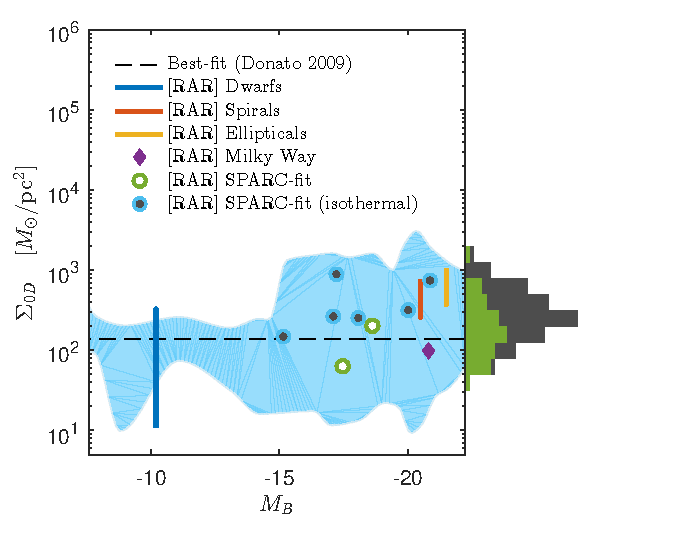
\includegraphics[width=0.9\hsize]{\ROOTPATH/fig.pdf}
	\caption{The different \textit{predicted} color lines correspond for each galaxy type showing the ability of the three parametric ($\beta_0,\theta_0,W_0$) RAR solutions for a particle mass $m c^2 \sim 50$~keV to be in agreement with the different $M_{\rm BH}-M_{\rm tot}$ relations considered in the literature (see \citet{RAR-II} for details) and explicited in the picture box. The RAR predictions for typical spirals (red) and ellipticals (yellow) together with the Milky Way solution (diamond) lay within the \textit{observable Ferrarese window}. The RAR prediction for typical dwarfs (blue) is located at the lower end of the $M_c$-$M_{\rm tot}$ plane, where data does not support. The black dots correspond to the critical core masses $M_c^{cr}$ while the black circle indicates the limiting maximum core mass for dwarfs $M_c^{\rm max}$. The SPARC results of this paper are presented in two groups. Green circles correspond to galaxies with total masses $M_{\rm tot} = M_s < 10^{14} M_\odot$, being $M_s$ the natural total mass of the obtained mass distribution. Light blue crosses correspond to total masses given by $M_{\rm tot} = M_b \ll M_s$,  being $M_b$ the mass at the boundary radius where the density falls to the critical density of the Local Group ($10^{-5} M_\odot/{\rm pc}^3$). Due to inappropriate halo information in the second group (light blue crosses) it is not possible to constrain the cutoff parameter $W_0$ what results in extended (isothermal) mass distributions with total masses $M_s \gg 10^{14} M_\odot$ which have to be truncated.}%
	\label{fig:SPARC:Ferrarese}%
\end{figure*}